\section{Agentic Training Framework}
\label{sec:agentic_training_framework}

% This section details the offline optimization module introduced in Section~\ref{sec:overview}. 
% We aim to train the agent to master the tree-based reasoning framework (Section~\ref{sec:tree_based_agentic_reasoning}) using Reinforcement Learning (RL). 
% However, training a robust ADP agent faces two fundamental challenges:
% (1) \textit{Reward Sparsity.} The strict syntactic requirements of operators and the binary nature of table correctness make positive feedback extremely rare during early training stages.
% (2) \textit{Data Scarcity.} Existing datasets lack the complexity of real-world ADP tasks, which involves long-horizon pipelines

% To address these challenges, we propose a {Progressive Agentic Training} framework. 
% First, to overcome reward sparsity, we design a {Cold-Start Curriculum} (Section~\ref{subsec:cold_start}) to initialize the agent's understanding of operator syntax and reasoning protocols, followed by a {Multi-turn RL} stage with a {Hybrid Reward} mechanism (Section~\ref{subsec:rl_reward}) that densifies feedback signals.
% Second, to address data scarcity, we develop a {Data Synthesis} engine (Section~\ref{subsec:data_synthesis}) that generates complex, high-quality training trajectories with realistic dirty data.

We propose a \emph{Progressive Agentic Training} framework for optimization. To mitigate reward sparsity, the framework includes a \emph{Cold-Start Curriculum} for initialization (Section~\ref{subsec:cold_start}), followed by a \emph{Multi-turn RL} stage with a \emph{Hybrid Reward} mechanism (Section~\ref{subsec:rl_reward}). To alleviate data scarcity, we develop a \emph{Data Synthesis} method (Section~\ref{subsec:data_synthesis}) that generates diverse ADP tasks for effective training.

\subsection{Cold-Start Curriculum}
\label{subsec:cold_start}

% %!TEX root = ../../main.tex
\begin{figure*}[t]
    \centering 
    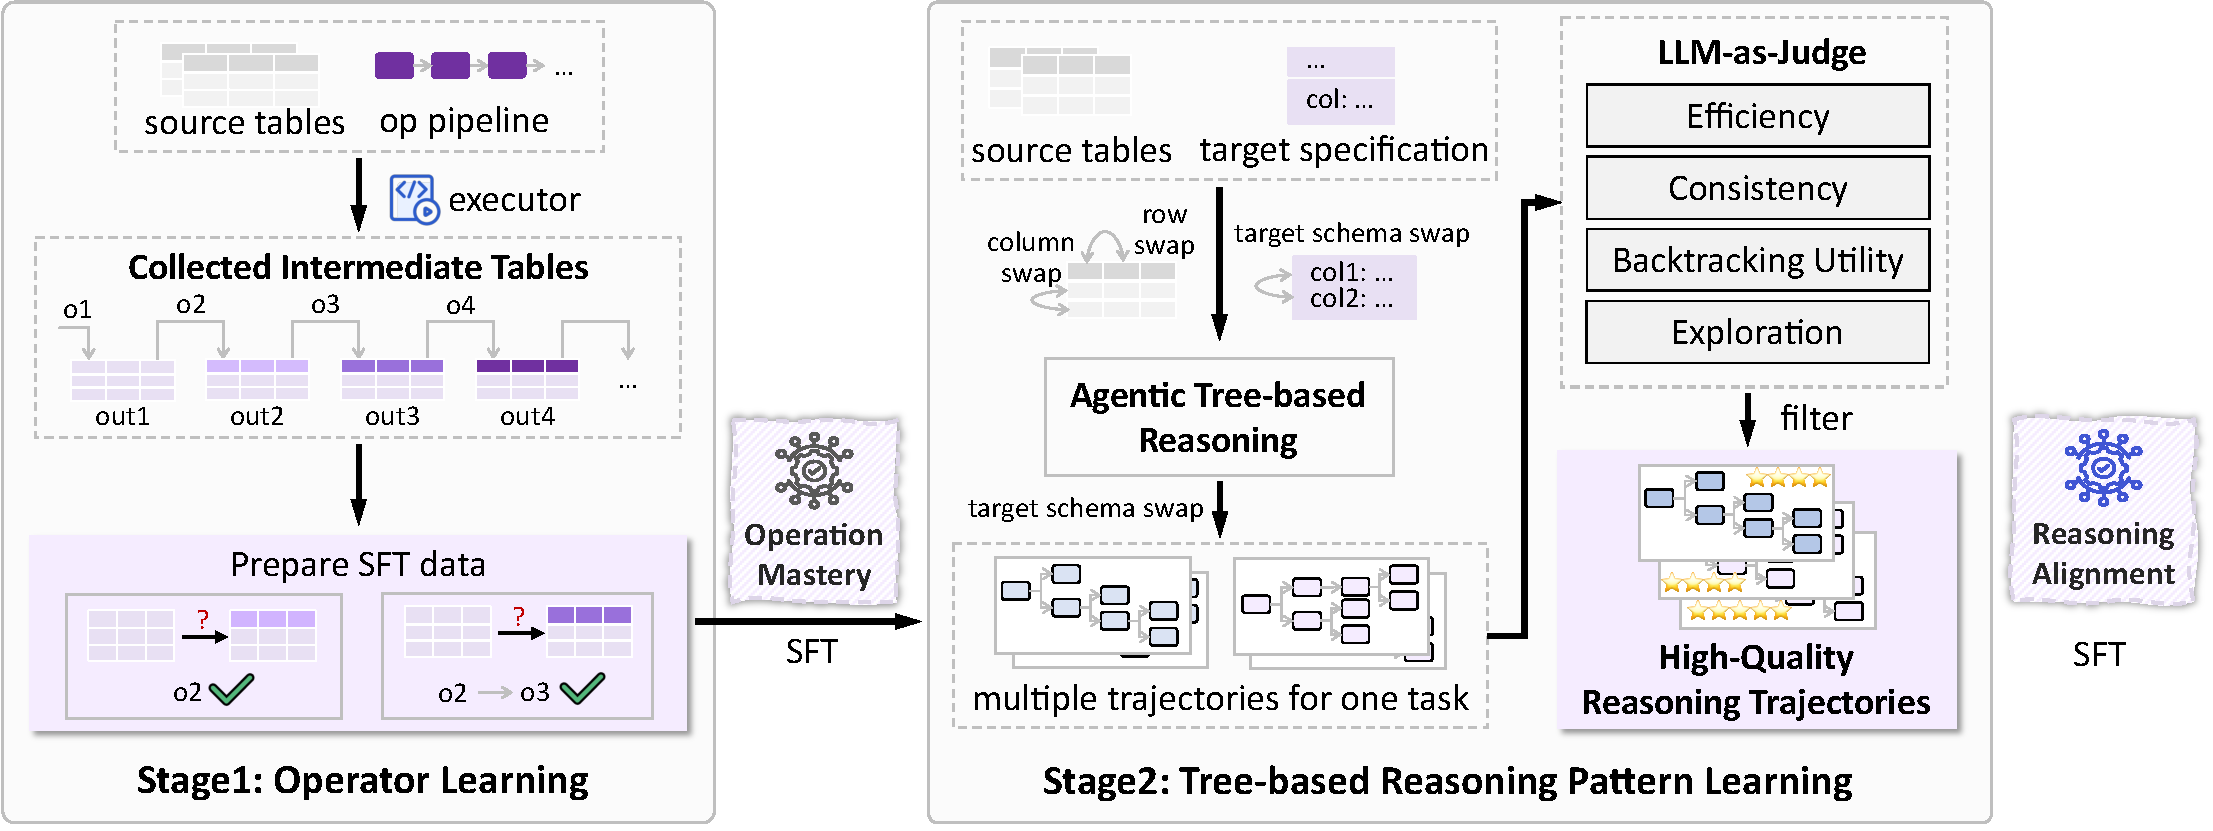
\includegraphics[width=0.9\textwidth]{figures/fig/cold_start.pdf}
  % \vspace{-0.7em}
    \caption{Overview of the progressive cold-start curriculum, which consists of two stages: Operator Learning and Multi-Solution Generation. An LLM-as-Judge mechanism filters these trajectories to ensure high-quality supervision for fine-tuning.
    }
    \label{fig:cold_start}
  % \vspace{-1em}
\end{figure*}

To mitigate the issue where an untrained LLM fails to produce executable pipelines, we design a Cold-Start Curriculum that initializes the LLM's reasoning capability for our structured and execution-grounded planning. 
Specifically, pre-trained LLMs generally lack an explicit understanding of operator syntax and the tree-based agentic reasoning procedure, which are previously described. Thus, without specialized supervision, the model cannot generate meaningful action sequences for ADP tasks. 
To address this, we employ a two-stage supervised fine-tuning (SFT) curriculum.

% The Cold-Start Curriculum addresses this through supervised fine-tuning (SFT) on curated examples that teach operator usage, planning decisions, and the interaction patterns. To this end, we design a two-stage SFT curriculum (Figure~\ref{fig:cold_start}) that targets operator syntax and reasoning procedures respectively.

%To mitigate the ``cold start'' problem where untrained agents fail to generate executable pipelines, we design a two-stage supervised fine-tuning (SFT) curriculum (Figure~\ref{fig:cold_start}) to instill operator syntax and reasoning protocols.

% To mitigate the ``cold start'' problem where an untrained agent fails to generate any executable pipeline during RL training, we design a two-stage supervised fine-tuning (SFT) curriculum before RL, as illustrated in Figure~\ref{fig:cold_start}. Tailored for ADP, we the cold start stage is designed to remember the operator syntax and tree-based reasoning protocol.

% \stitle{Stage 1: Operator Syntax Learning.}
% This stage focuses on the syntax and semantics of individual operators.
% Given source tables and a ground-truth operator pipeline $\mathcal{P}_{\text{total}}$ as defined in Eq.~(\ref{eq:pipeline_definition}), consisting a sequence of operators $(o_{\theta_i}^{(i)})_{i=1}^{k}$. We first execute these operators sequentially to collect a sequence of generated intermediate table sets $\{\mathcal{T}_{\theta_i}^{(i)}\}_{i=1}^{k}$ with Eq.~(\ref{eq:execute_pipeline}).
% Then, we sample a contiguous sub-sequence of operators $\mathcal{P}_{\text{sub}} = (o_{\theta_i}^{(i)}, \dots, o_{\theta_{i+k}}^{({i+k})})$ with corresponding input intermediate table set $\mathcal{T}_{\text{in}}=\mathcal{T}_{\theta_{i-1}}^{(i-1)}$ and output intermediate table set $\mathcal{T}_{\text{out}}=\mathcal{T}_{\theta_{i+k}}^{(i+k)}$.
% Through this way, we construct the operator syntax learning dataset consisting of a collection of training data pair $(\mathcal{P}_{\text{sub}}, \mathcal{T}_{\text{in}}, \mathcal{T}_{\text{out}})$, which .
% We conduct SFT conditioned on the data to optimize the loss $\mathcal{L}_{\text{op}}$:
% $$
% \mathcal{L}_{\text{op}} 
% = - \sum_{(\mathcal{T}_{\theta_{i-1}}^{(i-1)}, \mathcal{T}_{\theta_{i+k}}^{(i+k)}, \mathcal{P}_{\text{sub}}) \in \mathcal{D}_{\text{op}}}
% \log \Prob_{\text{LLM}}(
% \Serialize (\mathcal{P}_{\text{sub}})
% \mid 
% \Serialize (\mathcal{T}_{\theta_{i-1}}^{(i-1)}), \Serialize (\mathcal{T}_{\theta_{i+k}}^{(i+k)})
% ).
% $$



\stitle{Stage 1: Operator Syntax Learning.}
This stage focuses on the syntax and semantics of individual operators.
Given source tables and a ground-truth operator pipeline $\mathcal{P}_{\text{total}}$ as defined in Eq.~(\ref{eq:pipeline_definition}), consisting of a sequence of operators $(o^{(1)}, \dots, o^{(N)})$. We first execute these operators sequentially to collect a sequence of generated intermediate table sets $\{\mathcal{T}_{0}, \dots, \mathcal{T}_{N}\}$.
Then, we sample a contiguous sub-sequence of operators $\mathcal{P}_{\text{sub}} = (o^{(i)}, \dots, o^{(j)})$ with the corresponding input intermediate table set $\mathcal{T}_{\text{in}}=\mathcal{T}_{i-1}$ and output intermediate table set $\mathcal{T}_{\text{out}}=\mathcal{T}_{j}$.
In this way, we construct the operator syntax learning dataset $\mathcal{D}_{\text{op}}$ consisting of training triples $(\mathcal{P}_{\text{sub}}, \mathcal{T}_{\text{in}}, \mathcal{T}_{\text{out}})$.
Let $\phi(\cdot)$ denote the serialization function. It serializes $\mathcal{P}_{\text{sub}}$ by concatenating all serialized operators and intermediate table set $\mathcal{T}$ by serializing it into markdown format. We conduct SFT to optimize the following loss $\mathcal{L}_{\text{op}}$:
%
\begin{equation}
\label{eq:sft_op_learn}
\mathcal{L}_{\text{op}} 
= - \sum_{(\mathcal{P}_{\text{sub}}, \mathcal{T}_{\text{in}}, \mathcal{T}_{\text{out}}) \in \mathcal{D}_{\text{op}}}
\log \Prob_{\text{LLM}}(
\phi(\mathcal{P}_{\text{sub}})
\mid 
\phi(\mathcal{T}_{\text{in}}), \phi(\mathcal{T}_{\text{out}})
).
\end{equation}
%
Through Eq.~(\ref{eq:sft_op_learn}), the agent learns to recognize operator function signatures and argument formats, while isolating operator execution logic from higher-level planning decisions.
%This stage allows the model to master operator function signatures and argument formats, isolating execution logic from complex planning.
% \fanj{Definition mismatch issue: The conditional variables $T_{\text{in}}$ and $T_{\text{out}}$ are not formally defined in the preceding text, while the previously defined $\Pi_{\text{total}}$ does not appear in the objective. The formula should be aligned with the data construction description by explicitly defining $T_{\text{in}}$ and $T_{\text{out}}$, and clarifying how each training triple is derived from $\Pi_{\text{total}}$ (\eg via sub-sequence sampling and execution).}


% \stitle{Stage 2: Reasoning Procedure Learning.}
% This stage trains the model to follow the \textit{Agentic Tree-based Reasoning} mechanism (Section~\ref{subsec:agentic_tree_based_definition}), including the structured use of actions such as \action{plan} and \action{expand}.
% We construct a dataset of reasoning trajectories by distilling from strong teacher models (\eg DeepSeek-R1).
% For each ADP task with source tables $\mathcal{S}$ and target schema $\Sigma^\ast$, we aims to generate a high-quality tree-based agentic reasoning trajectories $\tau$.
% To improve robustness, input perturbations $\Phi$ are applied, \eg randomly shuffle the columns and rows for each source table.
% Then, we adopt in-Context Learning~\cite{dong2024survey}, which enables powerful LLMs to learn from few-shot examples without parameter update, on teacher models with a elaborate prompt to conduct tree-based learning following Eq.~(\ref{eq:overall_agentic_inference}). Finally, we collect a collection $\mathcal{U}$ of candidate trajectories $\tau=(R_1,R_2,\cdots,R_T,A)$
% These candidates are evaluated using a process reward function $R_{\text{llm}}(\tau)$ (Section~\ref{subsec:rl_reward}), and the top-ranked trajectories are retained as $\mathcal{U}^\ast$.
% The model is then fine-tuned to minimize...

\stitle{Stage 2: Reasoning Procedure Learning.}
This stage aligns the model with the \textit{Tree-based Agentic Reasoning} mechanism (Section~\ref{subsec:agentic_tree_based_definition}).
To achieve this, we synthesize a dataset of high-quality reasoning trajectories by distilling knowledge from strong teacher models (\eg DeepSeek-R1).
Specifically, for each ADP task defined by source tables $\mathcal{S}$ and a target schema $\Sigma^\ast$, we aim to generate a ground-truth trajectory $\tau$.
To enhance robustness, we apply input perturbations $\Phi$, such as randomly shuffling rows and columns in the source tables.
Next, we employ In-Context Learning~\cite{dong2024survey} to guide the teacher model. By utilizing elaborate prompts that exemplify the tree-based reasoning process defined in Eq.~(\ref{eq:overall_agentic_inference}), we generate a set of candidate trajectories $\mathcal{U}$.
To unify the training objective, we represent each trajectory as a sequence $\tau = (r_1, \dots, r_m)$. Here, the initial subsequence $(r_1, \dots, r_{m-1})$ corresponds to the iterative reasoning steps $(R_1, \dots, R_T)$ defined in Eq.~(\ref{eq:reasoning_process}), while the final element $r_m$ corresponds to the answer generation $A$ in Eq.~(\ref{eq:overall_agentic_inference}).
These candidates are filtered using a process reward function $R_{\text{llm}}(\tau)$ (detailed in Section~\ref{subsec:rl_reward}), and only the top-ranked trajectories are retained to form the final dataset $\mathcal{U}^\ast$.
Finally, the model is fine-tuned on $\mathcal{U}^\ast$ to minimize the masked negative log-likelihood:
%
\begin{equation}
\label{eq:sft_reasoning_learn}
\mathcal{L}_{\text{reason}} 
= - \sum_{\tau \in \mathcal{U}^\ast} 
\sum_{t=1}^{m} M_t \cdot \log \Prob_{\text{LLM}}(\phi(r_t) \mid \phi(r_{<t}), \phi(\mathcal{S}), \Sigma^\ast).
\end{equation}
%
Here, $r_t$ encapsulates both the current tree state and the agent's generated response. The serialization function $\phi(\cdot)$ transforms these structured components into a linear token sequence.
Crucially, we introduce a loss mask $M_t$ to ensure that gradients are only calculated for tokens corresponding to the agent's outputs.

% \fanj{How is $P_\theta(a_t \mid \mathcal{T}_t)$ defined?}

%This stage aligns the agent with the \textit{Agentic Tree-based Reasoning} protocol (Section~\ref{subsec:agentic_tree_based_definition}), specifically the usage of tags like \texttt{<plan} and \texttt{<expand}.
%We construct a dataset of high-quality reasoning trajectories by distilling from strong teacher models (\eg DeepSeek-R1).
%To ensure robustness, we apply input perturbations $\Phi$ to the training data and generate candidate trajectories $\mathcal{U}_{cand}$.
%We filter these candidates using an \textit{LLM-as-a-Judge} scoring function $Q(\tau)$ (detailed in Section~\ref{subsec:rl_reward}) and retain the top-ranked trajectories $\mathcal{U}_{filtered}$.
%The agent is then fine-tuned to minimize the negative log-likelihood of the actions $a_t$ given the tree state $\mathcal{T}_t$:
%$$
%\mathcal{L}_{\text{tree}}(\theta)
%= - \sum_{\tau \in \mathcal{U}_{filtered}}
%\sum_{t=1}^{|\tau|} \log P_\theta(a_t \mid \mathcal{T}_t).
%$$

\subsection{Multi-turn RL with Hybrid Reward}
\label{subsec:rl_reward}

\stitle{Motivation.}
Data preparation pipeline generation is a sequential decision process with execution feedback, where each action affects subsequent states and future operator choices. Optimizing such behavior cannot be reduced to single-shot generation. Instead, the policy should be trained over multi-turn interaction trajectories. In each turn, the agent produces structured actions (\eg \action{plan} and \action{expand}), the environment executes the proposed operators, and feedback is returned. Then, subsequent decisions are conditioned on these execution outcomes. 

\stitle{Basic Idea.}
The above setting motivates us to develop a multi-turn reinforcement learning method, where the policy is optimized over action sequences rather than single outputs. 
Specifically, under our interaction framework, each trajectory contains both (i) agent-generated tokens (actions and their contents) and (ii) environment-generated tokens, such as serialized intermediate tables and execution traces. In particular, since environment-generated tokens are deterministic execution outputs rather than policy decisions, they are excluded from policy gradient optimization. That is, we apply a binary token mask that removes gradients on tokens inside \action{execute} blocks, and optimize the policy only over agent decision tokens within \action{plan}, \action{expand}, and \action{answer}.

We optimize the policy using Group Relative Policy Optimization (GRPO)~\cite{shao2024deepseekmath}, which estimates baselines from group-level reward statistics, supporting more stable optimization over multi-turn trajectories. Using only final pipeline correctness as the reward, however, results in sparse and delayed learning signals. We therefore introduce a hybrid reward design, as described below.


%
%Different from single-shot generation, an ADP trajectory consists of multiple rounds of interaction.
%At each round, the agent outputs structured actions (\eg \action{plan} and \action{expand}), the environment executes the proposed operators, and returns deterministic feedback (\eg updated intermediate tables or error traces). 
%The agent then conditions on this feedback to make subsequent decisions.
%Formally, given a task input $x=(\mathcal{D},\mathcal{S})$, the policy $\pi_\theta$ induces a multi-turn trajectory $\tau$ that interleaves agent actions and environment observations until termination (\ie \action{answer}).
%
%\stitle{Masking Environment Observations.}
%In our interaction protocol, a trajectory contains both (i) agent-generated tokens (actions and their contents) and (ii) environment-generated tokens (observations), such as serialized intermediate tables and execution traces.
%Since the observation segments are deterministic outputs of the execution engine rather than the model's generative decisions, we mask them out during RL optimization.
%Concretely, we apply a binary token mask that zeroes gradients on all tokens inside observation blocks (\eg \action{execute}), and optimize the policy only on the agent decision tokens (\ie contents within \action{plan}, \action{expand}, and \action{answer}).

%\stitle{GRPO.} 
%We optimize the agent's policy with Group Relative Policy Optimization (GRPO)~\cite{shao2024deepseekmath}, which estimates baselines from group statistics instead of using a separate value network.

% \fanj{I have significantly revised the above paragraphs. Please check carefully.}

% We adopt the Group Relative Policy Optimization (GRPO) algorithm~\cite{shao2024deepseekmath} to optimize the agent's policy $\pi_\theta$. Unlike traditional PPO~\cite{schulman2017proximal} which requires a separate value function critic (often computationally expensive for long-context reasoning), GRPO estimates the baseline directly from group statistics.
% Formally, given an ADP task input $x = (\mathcal{D}, \mathcal{S}) \sim D$, we generate a group of $G$ trajectories (rollouts) $\tau = \{y_i\}_{i=1}^G$ sampled from the current policy $\pi_{\theta_{\text{old}}}$.
% For each trajectory $y_i$, we compute an advantage $A_i$ based on the reward function. The policy is optimized by maximizing the following objective:
% \begin{equation}
% \begin{split}
% \mathcal{J}(\theta) = \mathbb{E}_{x \sim D, \{y_i\}_{i=1}^G \sim \pi_{\theta_{\text{old}}}(\cdot|x)} 
% \frac{1}{G} \sum_{i=1}^G \bigg[ \min \bigg( \frac{\pi_\theta(y_i|x)}{\pi_{\theta_{\text{old}}}(y_i|x)} A_i, \\
% \text{clip} \left( \frac{\pi_\theta(y_i|x)}{\pi_{\theta_{\text{old}}}(y_i|x)}, 1-\epsilon, 1+\epsilon \right) A_i \bigg) - \beta \mathbb{D}_{\text{KL}} (\pi_\theta || \pi_{\theta_{\text{ref}}}) \bigg]
% \end{split}
% \end{equation}
% where $\epsilon$ is the clipping parameter to constrain the policy update, and $\pi_{\theta_{\text{ref}}}$ is the reference policy (typically the SFT model) used to prevent reward hacking via a KL-divergence penalty.

\stitle{Hybrid Reward.}
We design a hybrid reward mechanism that provides denser learning signals by evaluating both outcome quality and reasoning behavior. The overall reward $R(\tau)$ for a trajectory $\tau$ is defined as a weighted sum of three components:
%
\begin{equation}
    R(\tau) = \alpha \cdot R_{\text{out}}(\tau) + \beta \cdot R_{\text{part}}(\tau) + \gamma \cdot R_{\text{llm}}(\tau).
\end{equation}
%
where $R_{\text{out}}$, $R_{\text{part}}$, and $R_{\text{llm}}$ correspond to strict correctness, partial progress, and reasoning process signals, respectively, and $\alpha, \beta, \gamma$ are hyperparameters that balance their contributions. 
Now, we detail each of the three components $R_{\text{out}}$, $R_{\text{part}}$, and $R_{\text{llm}}$ as follows. 

%we design a {Hybrid Reward} mechanism that densifies the feedback signal by assessing both the {outcome quality} and the {reasoning process}. The total reward $R(\tau)$ for a trajectory $\tau$ is defined as a weighted sum of three components:
%\begin{equation}
%    R(\tau) = \alpha \cdot R_{\text{out}}(\tau) + \beta \cdot R_{\text{partial}}(\tau) + %\gamma \cdot R_{\text{llm}}(\tau),
%\end{equation}
%where $\alpha, \beta, \gamma$ are hyperparameters balancing strict correctness, partial progress, and reasoning quality. We detail each component below.

\etitle{Outcome Reward $R_{\text{out}}$.}
This reward provides a direct success signal based on final output correctness. When the \action{answer} action is issued, the generated resulting target table $\hat{T}$ is evaluated by:
\begin{equation}
R_{\text{out}}(\tau) = \mathbb{I}(\hat{T} \equiv T^*).
\end{equation}
where $\mathbb{I}(\cdot)$ denotes the indicator function.


%\etitle{Outcome Reward $R_{\text{out}}$.}
%$R_{\text{out}}$ serves as the strict success signal. When the agent triggers the \texttt{<terminate} action, we extract the table $\hat{T}$ from the selected leaf node.
%$$
%R_{\text{out}}(\tau) = \mathbb{I}(\hat{T} \equiv T^*),
%$$
%where $\mathbb{I}(\cdot)$ is the indicator function.

\etitle{Partial Reward $R_{\text{part}}$.}
This reward provides a partial-progress signal when strict correctness is not achieved ($R_{\text{out}}(\tau)=0$). We measure the similarity between the generated table $\hat{T}$ and ground-truth $T^*$, and define $R_{\text{part}}(\tau) = \texttt{avg}(S_{sch}, S_{shp}, S_{cnt})$, where $S_{sch}, S_{shp}, S_{cnt}$ evaluate alignment in schema, shape and content, respectively:
%
\begin{equation} 
% \nonumber
\begin{aligned}
S_{sch} &= \frac{|C_{\hat{T}} \cap C_{T^*}|}{|C_{\hat{T}} \cup C_{T^*}|}, \quad
S_{shp} = \exp\!\left(- \left| \frac{|\hat{D}| - |D^*|}{|D^*|} \right| \right), \\
S_{cnt} &= \frac{1}{|C_{m}|} \sum_{c \in C_{m}} \frac{\sum_{i} \mathbb{I}(\hat{D}[c]_i = D^*[c]_i)}{\max(|\hat{D}|, |D^*|)}.
\end{aligned}
\end{equation}


%
%\etitle{Partial Reward}
%$R_{\text{partial}}$ guides exploration when $R_{\text{out}}=0$, we quantify the similarity between the generated table $\hat{T}$ and $T^*$ to provide dense gradient signals. We define $R_{\text{partial}} = \frac{1}{3}(S_{sch} + S_{shp} + S_{cnt})$, where the three components measure alignment across schema, shape, and content dimensions respectively:
%
%
%\begin{equation}
%\begin{aligned}
%S_{sch} &= \frac{|C_{\hat{T}} \cap C_{T^*}|}{|C_{\hat{T}} \cup C_{T^*}|}, \quad
%S_{shp} = \exp\left(- \left| \frac{|\hat{D}| - |D^*|}{|D^*|} \right| \right), \\
%S_{cnt} &= \frac{1}{|C_{m}|} \sum_{c \in C_{m}} \frac{\sum_{i} \mathbb{I}(\hat{D}[c]_i = %D^*[c]_i)}{\max(|\hat{D}|, |D^*|)}.
%\end{aligned}
%\end{equation}
%

Here, $C_{\hat{T}}$ and $C_{T^\ast}$ denote the column-name sets, $|\hat{D}|$ and $|D^\ast|$ denote the row counts, and $C_{m} = C_{\hat{T}} \cap C_{T^*}$ is the set of matched columns used for cell-wise value comparison.
%
%Here, $C_{\hat{T}}$ and $C_{T^*}$ denote the column name sets, $|\hat{D}|$ and $|D^*|$ denote the row counts, and $C_{m} = C_{\hat{T}} \cap C_{T^*}$ represents the set of matched columns used for cell-wise value comparison.

\etitle{Process Reward $R_{\text{llm}}$}.
Relying solely on data similarity rewards may lead to \emph{reward hacking}, which has been studied in other reinforcement learning settings~\cite{taylor2025school,zhang2025reward}, and can also arise in ADP scenarios (\eg renaming columns without performing the required data cleaning).
To discourage such ``shortcut'' strategies,
% and promote semantically consistent decision-making, 
we introduce a process reward that evaluates the quality of the reasoning trajectory. We use an instruction-tuned LLM (\eg GPT-4o) as a judge to score each trajectory based on the actions defined in Section~\ref{sec:tree_based_agentic_reasoning}. 

Specifically, the judge evaluates three criteria:
(1) \textit{Plan–action consistency}, measuring whether generated pipeline (from \action{expand}) correctly implements the plan (from \action{plan}).
(2) \textit{Feedback responsiveness}, checking whether subsequent \action{plan} outputs explicitly respond to the prior execution feedback (\eg reported error traces).
(3) \textit{Backtracking justification}, verifying that parent-node switches are supported by recorded failure evidence from the current branch.


%Relying solely on data similarity can lead to "reward hacking" (\eg renaming columns without cleaning data). To enforce robust decision-making, we introduce a process-based reward $R_{\text{reason}}$ that evaluates the semantic coherence of the generated tree nodes.
%We employ a frozen, instruction-tuned LLM (\eg GPT-4o) as a judge to score the trajectory based on the node components defined in Section~\ref{sec:tree_based_agentic_reasoning}.
%The judge evaluates three specific criteria: (1) \textit{Plan-Action Consistency}, checking if the generated operator sequence $\Delta \Pi$ faithfully implements the reasoning plan $\psi$; (2) \textit{Feedback Responsiveness}, ensuring that if a node contains negative feedback (\eg error traceback in $\eta$), the subsequent plan $\psi_{new}$ explicitly acknowledges and addresses it; and (3) \textit{Backtracking Justification}, verifying that decisions to switch parent nodes are logically justified by the failure of the current branch. The final $R_{\text{reason}}$ is the average score of these three dimensions.

\subsection{Data Synthesis for Training}
\label{subsec:data_synthesis}
To train our agentic model, we require supervision in the form of executable data preparation pipelines together with their source and target tables. Since such ADP task instances are not available at scale, we construct them through synthesis by converting SQL benchmarks into ADP tasks consisting of source tables, a target table, and a corresponding transformation pipeline.
%
Synthesizing such training tasks has two key challenges. First, the generated pipelines should correspond to meaningful analytical transformations rather than arbitrary operator chains, so that the supervision reflects realistic operator dependencies. Second, the synthesized source tables should include diverse data quality issues while preserving the intended transformation logic. Excessive noise injection may break key fields or relationships~\cite{rekatsinas2017holoclean}, making it difficult to construct any feasible pipeline that produces the target table.

\stitle{ADP Task Construction from NL2SQL.}
To obtain realistic ADP tasks, we instantiate them from NL2SQL benchmarks~\cite{spider_dataset,bird_dataset}.
% , which provide real databases paired with analytical SQL queries. 
For each query $q$, we execute it to produce the target table $T^*$ and use an LLM to generate the corresponding target schema specification. We also translate $q$ into an operator pipeline by generating candidate pipelines with an LLM and selecting the shortest one that exactly reproduces $T^*$ through execution. This yields a clean task instance consisting of source tables, a target schema specification, a target table, and an operator pipeline.

\stitle{Reversible Noise Injection.}
Since NL2SQL data is typically clean, we introduce controlled noise to increase data diversity for training. We inject noise by applying inverse transformations of data-cleaning operators, so that each corruption corresponds to a valid cleaning step. Specifically, we sample an operator and use an LLM to generate its inverse transformation logic. For example, the inverse of a date-standardization operator converts a normalized date (\eg ``2023-01-01'') into heterogeneous formats (\eg ``01/01/23''). After each corruption step, we verify executability by applying the corresponding cleaning operator and checking that the previous table state is restored. Only reversible corruptions are kept. Repeating this process produces dirty source tables together with a matching cleaning pipeline. The final ground-truth pipeline is formed by concatenating the cleaning pipeline with the task pipeline.
